\chapter{系统硬件平台设计}
低功耗海洋传感器集成系统将集成多种海洋传感器,主要目的是针对传感器进行有效管理。系统在低功耗的指标下可通过对传感器下达控制和工作指令从而获取海洋水文数据的采集,数据可进行本地存储,也可通过预留接口对传感器采样数据进行回收。系统硬件平台    主要由传感器连接控制模块和微处理器模块两大部分组成。其电子电路的设计上主要受系统稳定性、系统功耗和电路板PCB大小限制,在保证功能稳定的前提下,应该优先选择具备功耗控制功能和较小封装的外设芯片以确保系统的电子电路在规定的有限舱体内长时间稳定工作。整个硬件设计在稳定性和低功耗性方面做大量研究,实现安全可靠的硬件观测平台,为系统的稳定运行提供保障。
\section{传感器连接控制模块}
传感器连接控制模块主要负责各海洋传感器的管理工作及状态监控等,具体包括传感器电源控制、数据通信协议转换等,电源控制部分设计关键在于需要根据不同传感器负载选用不同型号的DC/DC电压转换模块,经由微处理器来控制其开关;传感器数据通信部分主要使用了串行设备通信协议,根据本文中的传感器数据传输协议~\cite{2017jy}和接口类型,在该模块中,AML系列海洋传感器都统一使用AML专用的传输协议,其他类型传感器主要采用了RS232或RS485接口进行通信,传感器模块给微处理器传输状态信息和采样数据,同时微处理器也可以经过该方式给传感器下达传感器配置、采样、查询等命令。
\subsection{电源供应与分配部分}
由于整个系统各个模块所需求的电压不同,所以对接入电压需进行合理的转换分配,以满足各模块的正常工作。在电子电路中设计了电压转换电路可以避免使用多个电压源造成电池能源和舱体空间的浪费。为了达到低功耗的要求,给海洋传感器供电时应考虑可控性。因而采用控制式的DC/DC电压转化模块,用于实现对海洋传感器的上电与断电。

对于DC/DC模块的选用,主要依据于各个模块、器件所需工作电压和工作功率的要求。为了保证各电子器件能够工作,需要将接入电压~\cite{yzx}转换成各器件所需的工作电压,比如9V、5V或3.3V等。低功耗海洋传感器集成系统的能源都是来自于携带的电池组,电池组由七节锂电池串联而成,每节锂电池的电压范围是:3.8\-4.2V。由于锂电池随着电池容量的变化,电压也会出现变化,这也要求DC/DC模块具备宽输入电压。系统的处理器MSP430F5438A和其他模块芯片所需要的正常工作电压是3.3v。因此需要将接入电压转化为3.3V,主要通过相对应的DC/DC电压转化模块来完成,相关电路原理图如图~\ref{fig:DC3.3V}所示。

\begin{figure*}[ht]
    \centering
	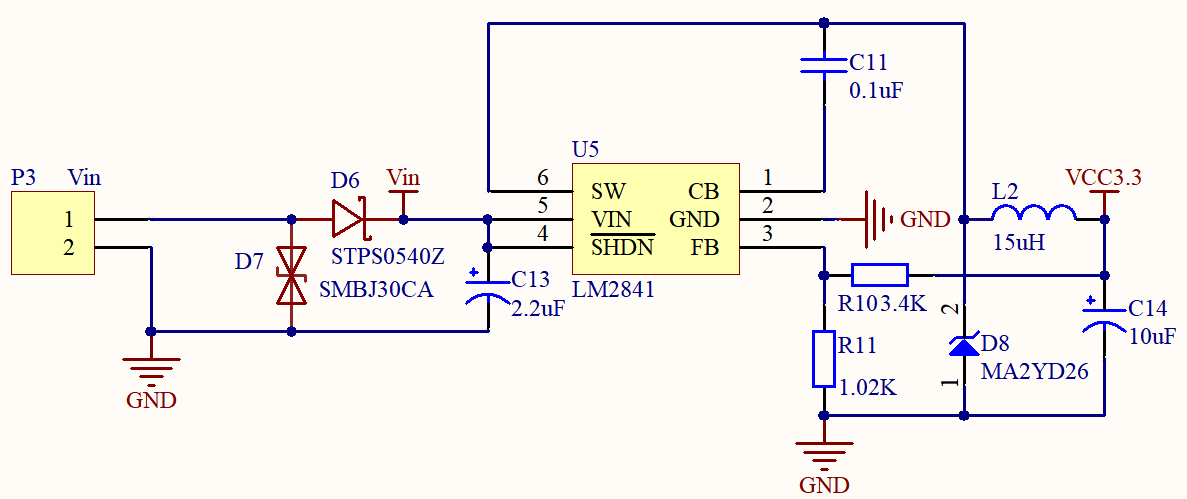
\includegraphics[width=0.8\textwidth]{fig/DC_3.3.png}
	\caption{转DC3.3V电路原理图}
	\label{fig:DC3.3V}
\end{figure*}
                                                
DC/DC电压转化模块选用了TI公司的LM2841,这款DC/DC降压调节器的输入电压范围从4.5V到42V,输出电流300mA,适合于广泛的应用。最大效率可达85\%,同时具有软启动的功能可实现控制上电断电(SHND引脚拉到GND以禁用设备,拉高以启动设备)。输出电压可设置,通过公式\ref{eq:功率}可计算输出电压,根据实际需要的电压,来设置R10和R11的电阻比。
\begin{equation}
\begin{split}
\mathcal{V}_{OUT} = 0.765 V (1 + (R10/ R11))
\end{split}
\label{eq:功率}
\end{equation}   

通常,R11被赋予100Ω到10kΩ的起始值。

\subsection{传感器电源管理部分}
对于海洋传感器的供电问题,将使用DC/DC电源模块将接入的电源电压转换为海洋传感器正常工作需要的电压(9V)为其供电。海洋传感器的电源管理使用带有Ctrl端可控的隔离稳压电源模块,从MSP430控制芯片下达控制指令,对传感器进行上电和断电的操作。将接入电压转9V的具体电路实现如图~\ref{fig:DC9V}所示。

\begin{figure*}[ht]
    \centering
	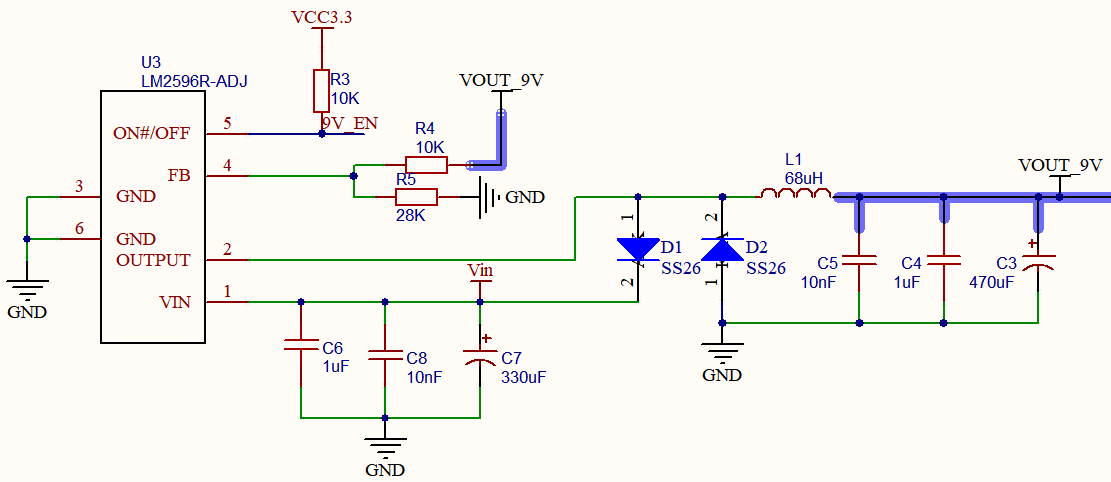
\includegraphics[width=0.8\textwidth]{fig/DC_9V.png}
	\caption{转DC9V电路原理图}
	\label{fig:DC9V}
\end{figure*}

电子电路设计中使用了LM2596降压DCDC芯片,其具有程序可控、输出效率高、宽输入电压范围、输出过压保护、过流保护以及短路保护的特点。高效率、大电流、低纹波的特点满足设计要求。可实现将DC12V输入转9V,同时较大的输出电流,也能够满足多个传感器负载。

\subsection{传感器数据通信部分}
该部分实现的功能主要是将不同传感器的通信方式转换为能够直接与微控制器相连的电平信号,本系统为微处理与海洋传感器连接提供了两种数据通信协议,其一为常用的RS232通信协议标准(一种点对点的数据传输方式),使用较为简单,只需将TX、RX、GND进行连接后即可完成相关的通信流程;其二是与AML系统海洋传感器连接的特定协议。

\subsubsection{RS232协议转换部分}
微处理器与海洋海洋传感器通信接口采用RS232标准。RS232协议支持全双工传输数据,其通信标准可以以九针接口定义,也可以使用三针接口定义~\cite{2020xxw}。本设计使用三针的接口定义,只需要使用TX、RX、GND三个引脚,利用MAX323SE实现TTL电平到RS232电平的转换,该芯片具有较好的低功耗性能,供电范围为3V-5.5V。具体电路实现如图~\ref{fig:RS232}所示。

\begin{figure*}[ht]
    \centering
	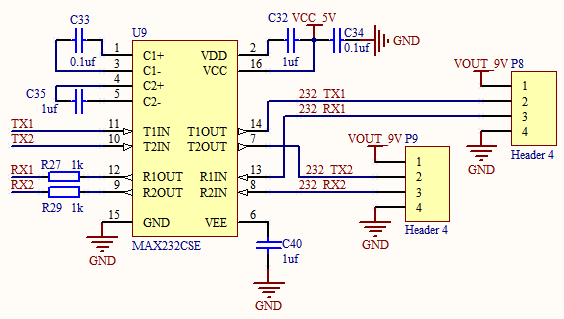
\includegraphics[width=0.8\textwidth]{fig/RS232.png}
	\caption{电平转换电路}
	\label{fig:RS232}
\end{figure*}

对于不同接口的海洋传感器,如RS422或RS485通信接口,可以选用相应型号的转换芯片来支持对应的接口。

\subsubsection{AML传感器连接部分}
AML\uline{ }Xchange系列传感器需要特定的电气协议和数据接口与设备连接,所有的AML智能传感器共享相同的电源。AML\_ Xchange系列传感器通过特定的传感器接口与OEM板连接,OEM板再与微处理器之间直接进行通信(TTL电平协议通信)。OEM板连接图如图~\ref{fig:OEM板连接图}所示:

\begin{figure*}[ht]
    \centering
	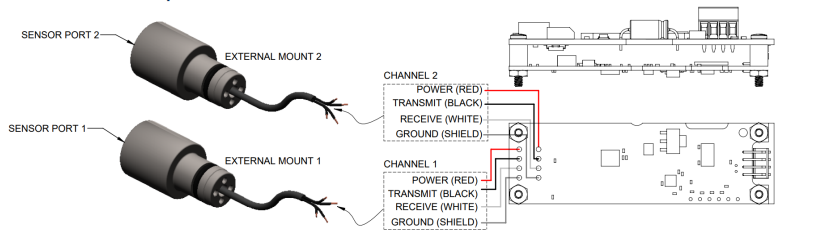
\includegraphics[width=\textwidth]{fig/OEM板连接图.png}
	\caption{OEM板连接图}
	\label{fig:OEM板连接图}
\end{figure*}

每块OEM板上有两个传感器通道,通道有电源、地、接收、发送四个引脚。OEM板接上传感器接口后,AML\_Xchange系列传感器插头旋拧进接口就形成了完整的连接。AML\_Xchange系列传感器插头实物如图~\ref{fig:AMLXchange}所示。

\begin{figure*}[ht]
    \centering
	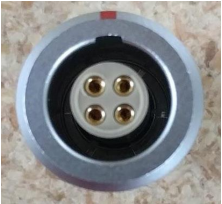
\includegraphics[width=0.3\textwidth]{fig/AML_Xchange.png}
	\caption{AML\uline{ }Xchange系列传感器插头}
	\label{fig:AMLXchange}
\end{figure*}

由于不同类型传感器共享相同的电源,且接口是一致的。如需更换传感器的类型,将其从OEM板接口拧出,更换上相应的传感器即可。

\section{微处理器模块}
微处理器模块是整个平台最为核心的部分,是系统完成各项功能的控制中心,承载着水下所有数据采集任务。该模块主要由MSP430F5438A控制芯片构成的最小系统、串口拓展电路、数据存储电路以及数据回收接口电路组成。
\subsection{最小系统}
最小系统主要由MSP430F5438A微处理器芯片、时钟电路、复位电路和下载电路组成。TI MSP系列超低功耗控制器种类繁多,可针对不同的应用需求进行选择。该微处理器具有优越的低功耗性能,当系统不需要进行工作任务时可根据最低电源消耗、最快速启动时间和可用唤醒源选择进入某一种低功耗模式。在系统处于非任务状态下配置成LPM3低功耗模式,该模式下功耗典型值小于2uA。MSP430具体架构如图~\ref{fig:MSP430架构}所示:

\begin{figure*}[ht]
    \centering
	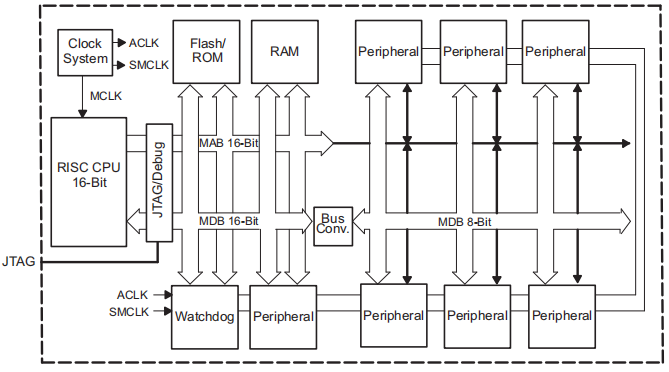
\includegraphics[width=0.8\textwidth]{fig/MSP430架构.png}
	\caption{MSP430架构}
	\label{fig:MSP430架构}
\end{figure*}

\subsubsection{微处理器时钟系统} 
从最基本的时钟系统出发,能够直观的理解MSP430F5438A这款微处理器芯片。这里对时钟系统进行简要的介绍。标准时钟系统(Unified Clock System(UCS))可以为芯片提供各种所需的时钟信号。MSP430F5438A的UCS模块由主系统时钟(MCLK)、子系统时钟(SMCLK)、辅助时钟(ACLK)以及专用时钟(MODCLK)这四个时钟系统组成~\cite{sxf}。

本系统的外部高速晶体振荡电路采用16MHZ的高速晶振,晶振连接到XT2IN和XT2OUT。但是上电后,XT2会一直保持静止状态,直到通过PSEL设置成XT2模式,PSEL置位,XT2IN和XT2OUT将配置成XT2模式。如果与XT2IN对应的PSEL位清零,XT2IN和XT2OUT均会被配置为普通的IO口模式,此时XT2的功能是禁止的。外部高速时钟源电路如图~\ref{fig:外部时钟源电路}所示:

\begin{figure*}[ht]
    \centering
	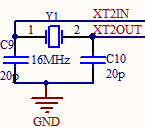
\includegraphics[width=0.5\textwidth]{fig/外部时钟源电路.png}
	\caption{外部高速时钟源电路}
	\label{fig:外部时钟源电路}
\end{figure*} 

\subsubsection{下载电路} 
进行软件调试时,通常会直接烧写程序或者在线仿真,仿真和烧写有几种方式可供选择。最常见的是JTAG方式,可以访问到MSP430所有资源。JTAG既可以对MSP430进行仿真也可以编程,需要使用的主要连线有TMS、TCK、TDI、TDO。图~\ref{fig:JTAG接口定义图}是JTAG的接口定义图。

\begin{figure*}[ht]
    \centering
	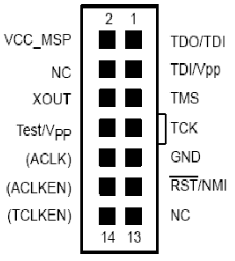
\includegraphics[width=0.4\textwidth]{fig/JTAG接口定义图.png}
	\caption{JTAG接口定义图}
	\label{fig:JTAG接口定义图}
\end{figure*}


SBW(SPY-BI-WIRE)又简称为两线制JTAG,只需要SBWTCK、SBWTDIO这两根线路。SBW既可以留有更多的IO资源,也可以让设计的PCB板更加小型化。电子电路设计中,在满足性能指标的情况下,尽可能选择简化设计的方法,对于本系统的微型化设计的目标具有重要的意义。下载电路如图~\ref{fig:下载电路}所示:

\begin{figure*}[ht]
    \centering
	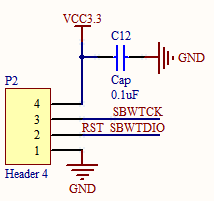
\includegraphics[width=0.5\textwidth]{fig/下载电路.png}
	\caption{下载电路}
	\label{fig:下载电路}
\end{figure*}

\subsubsection{外部复位电路}
嵌入式微处理器MSP430F5438A的内部复位信号在NRST引脚上,内部的脉冲发生器保证每一个复位源有20us的脉冲延时,当NRST引脚被拉低产生外部复位信号时。硬件原理图如图~\ref{fig:外部复位电路}所示。
\begin{figure*}[ht]
    \centering
	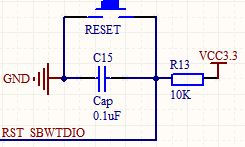
\includegraphics[width=0.5\textwidth]{fig/外部复位电路.png}
	\caption{外部复位电路}
	\label{fig:外部复位电路}
\end{figure*}

\subsubsection{实时钟电路}
本系统需要长期工作于深海环境之下,在甲板上设置好参数之后,从设备投放海底到回收期间,系统会自动化的采集海洋水文数据,相关的外部工作人员除非出现设备故障,否则不会有工作人员对系统设备进行干预。一方面在电源管理的部分,需要定时周期性的给电子设备和海洋传感器设备进行供电;另外一方面,在进行数据采集时,需要加上时间戳并且各种不同的海洋水文数据需要同步测得,这种数据采集才具备研究的价值和意义。高精度实时钟能够在系统参数配置的阶段接受到工作人员发送来的系统时间,从设定的系统时间开始计时。程序可以记录上一次数据采集的时间,并计算下一次数据采集的时间。

MSP430F5438A是自带实时钟模块(RTC)的,提供带日历、可编程闹钟和校准功能的时钟计数器。供电引脚VBAT脚采用混合供电的方式,由CR2110纽扣电池和3.3V电池同时供电,确保RTC的运行。RTC\_A模块是计数增加的时钟源可以是ACLK、SMCLK或者是分频之后的ACLK或者SMCLK。为了方便RTC\_A日历的操作,ACLK必须设置为32768Hz(通常情况)。由于时钟源不论是选择内部时钟,还有选择外部晶振产生的时钟都会产生比较大的时间误差。

低功耗海洋传感器集成系统是铺设在海底环境当中的,进行数据采集记录时间戳需要较为精准的时间。如果要外部的工作人员去进行时间校准的话成本会很大,所以对于实时钟的时间准确度和稳定性是有极高的要求的。本系统选用了极端精确的带有集成晶体和SRAM的SPI总线时钟芯片DS3234。为确保电路的稳定性和安全性同时提高CS和INT的高电平输出能力,分别在片选线和中断触发上接10k上拉电阻。具体的电路实现如图~\ref{fig:高精度实时钟电路}所示:

\begin{figure*}[ht]
    \centering
	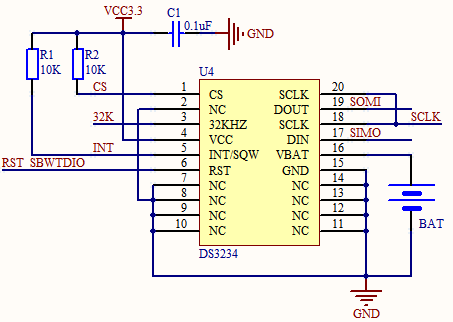
\includegraphics[width=0.6\textwidth]{fig/高精度实时钟模块电路.png}
	\caption{高精度实时钟电路}
	\label{fig:高精度实时钟电路}
\end{figure*}

DS3234具有低成本、高精度的优点。它可以提供一个稳定而精确的参考时钟,误差在每年2分钟之内。通过SPI总线的方式与MSP430微控制器进行通信。DS3234作为SPI串行总线的从设备,通过CS脚进行片选。DS3234数据传输方式具有很大的灵活性,支持单字节和多字节两种数据传输。在32K这个引脚上可以输出一个稳定32KHZ频率的时钟源给到MSP430微控制器。DS3234具备闹钟的功能,当系统时间与设定的闹钟时间达到一致时,在INT/SQW引脚上会产生一个中断信号给微处理器。

\subsection{串口拓展电路}
串口通信在计算机、工业控制、自动化等领域应用广泛,常见的串口通信协议有RS232、RS422、RS485等,都是各仪器设备通用的通信协议。RS232通信协议使用比较简单,通信速率较低,通信距离一般不超过25米,通常用于点对点的数据传输;RS422采用平衡方式传输,根据两条传输线之间的差分信号来判断逻辑状态,拥有比RS232更强的驱动能力~\cite{2020wqh}。RS485串口通信可实现2线半双工和4线全双工,传输距离可达1.2Km,现在多采用两线制方式,这种总线式拓扑结构可实现同时挂接32个以上设备,可实现一主多从的通信方式~\cite{2016cmy}。MSP430F5438A微处理器自身具有4个普通串口(UART)。

根据系统要求,海洋传感器需要普通串口四路(每路具有两个通道),还要有两路作为备用,所搭载的海洋传感器多为AML系列,其它的海洋传感器通信方式都为RS232串行通信,为了满足多种类型海洋传感器集成搭载的需求,因而对串口资源进行了拓展。

\begin{figure*}[ht]
    \centering
	\includegraphics[width=0.7\textwidth]{fig/wk2124.png}
	\caption{串口拓展电路}
	\label{fig:串口拓展电路}
\end{figure*}

本文所采用的拓展芯片为成都为开微电子公司的WK2124。WK2124采用的是SPI接口,有四个通道的UART。它是低功耗设计,可以配置为自动休眠、微秒级自动唤醒模式。主UART支持波特率自动适应,宽工作电压设计2.5V\-5V,各UART通道都有与之对应的寄存器和控制字,方便对各通道进行控制。

WK2124的主接口接到MSP430F5438A的SPI总线,需要MOSI、MISO、VCC和GND四根线进行连接即可,通过SPI总线协议转UART协议进行数据通信。需要注意的是,上电复位后,WK2124需要先写入OX55,其可以自动测得微处理器的波特率,并锁定主UART的波特率,之后WK2124和主机的通信就按照此波特率进行;如果需要更换其他的波特率,则需要对芯片进行硬件复位操作,然后在进行波特率测试和锁定。WK2124具体的电路实现如图~\ref{fig:串口拓展电路}所示:

WK2124采用+3.3V供电,RST是硬件复位引脚,低电平有效,复位期间及复位后,各子串口处于禁止收发状态,当子串口处于联网状态下,该特性使得该子串口所在的子节点在上电、复位期间不会对联网的其他子节点产生干扰。此外,各子串口也可以实现软件复位。RST\_SBWTDIO节点也可以接微处理器芯片的普通I/O引脚,用于通电期间的复位操作。

WK2124的中断输出引脚IRQ一般接微处理器的外部中断引脚。WK2124有两级中断:子串口中断和全局中断。全局中断寄存器GIFR用以判断中断类型,然后在相应的中断状态寄存器中可以读取到当前的中断源。此外,WK2124的每个子串口都有独立的中断系统,包括FIFO数据错误中断,发送FIFO触发点中断等。中断被使能以后,满足中断触发条件就会触发对应的中断。

\subsection{数据存储电路}
在低功耗海洋传感器集成系统中,可以把采集到的海洋水文数据存储于TF卡中。SD卡是一种便携的可移动存储设备,数据传输快、支持热插拔。TF卡,又称Micro SD卡,体积约是SD卡的1/4,和SD卡相比体积较小,适于小巧或空间有限的设备使用。

TF卡和SD卡的通信协议和编码地址都是一样的,通信协议为SPI总线~\cite{2015zjh}和SD总线,虽功能相同,但接口不同。TF卡的优势不言而喻,在实际开发和应用中,占据物理空间更小的TF卡会得到更广泛的使用。SPI总线相比SD总线虽有通信速率上的不足,但是也很明显的优势就是简化主机的设计。

在本系统中主机和TF卡之间选取了SPI总线进行数据通信。这是出于两个方面考虑的:MSP430F5438A微控制器的SD模式引脚被其它模块所占用,为了简化主机的设计和节省微处理器资源;SPI总线的数据通信速率是能够满足海洋传感器集成系统中数据采集的要求的。

TF卡存储电路实现原理图如图~\ref{fig:TF卡电路}所示:

\begin{figure*}[ht]
    \centering
	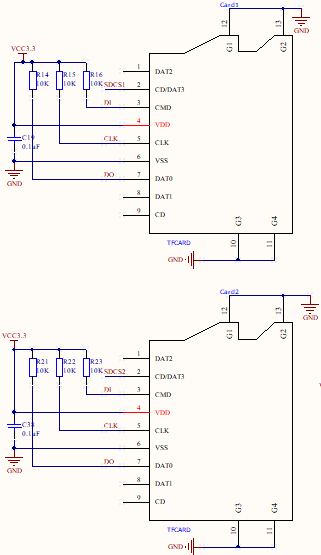
\includegraphics[width=0.5\textwidth]{fig/TF卡电路.png}
	\caption{数据存储电路}
	\label{fig:TF卡电路}
\end{figure*}

系统中采用TF卡的主要作用就是将海洋传感器数据存储于TF卡当中。此功能和USB挂载硬盘类似,但是用TF卡功耗比较小,所占物理空间也比硬盘小得多。虽然系统在海底环境需要长期进行采样,但是数据采集不是连续的。数据储存量要求并没有太高,用TF卡是能够满足储存采集数据要求的。
\subsection{数据回收电路}
低功耗海洋传感器集成系统中采集到的海洋水文数据,一方面可以通过本地存储保存在TF卡中,另一方面可以通过预留出接口把数据进行回收。本系统设计采用CH340E芯片将串口转成USB接口方便用来进行调试和回收采集数据。当设备从海洋环境当中打捞出来时,个人计算机只要接上USB线就能便捷的获取海洋传感器采集数据和整个系统的状态;系统出现故障时,维修人员将系统设备从海底打捞上来,接上USB接口也能及时进行系统调试,对于系统的现场维护具有重要意义。具体的USB接口电路实现如图~\ref{fig:USB接口模块原理图}所示。

\begin{figure*}[ht]
    \centering
	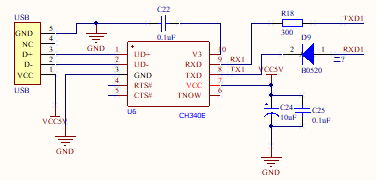
\includegraphics[width=0.7\textwidth]{fig/usb.png}
	\caption{USB接口电路原理图}
	\label{fig:USB接口模块原理图}
\end{figure*}

本模块选用串口转USB芯片CH340E,可实现串口转USB。CH340E芯片只有10个引脚,简化设计的同时还节省了设备的空间。从原理图~\ref{fig:USB接口模块原理图}中可以看出MSP430F5438A的串口一升级成USB总线。计算机通过USB总线与微处理器控制板进行连接,方便进行串口测试,另外可使用USB总线直接进行串口下载程序。所以USB接口模块很大程度上优化了系统的测试和使用便捷性。

\section{可靠性和冗余设计}
系统中采集到的海洋水文数据进行储存时,主机对TF卡可能既要进行读操作又要进行写操作。但是从以往实际应用TF卡存储的经验中发现:在进行读写操作时,读写可能不稳定从而导致数据会出现丢失的情况。从原理图~\ref{fig:TF卡电路}中可以看到,TF卡存储模块采用了冗余设计。在对TF卡进行写时,进行两次写操作,数据既要写入到TF卡一当中,又要写入到TF卡二当中。其中一块存储卡写发生故障或者数据丢失时,仍能够保证数据安全的本地保存。这样做的好处是,提高系统的可靠性,通过备份的手段,保证了数据读写的稳定性,增强系统的鲁棒性。


\section{本章小结}
本章阐述了低功耗海洋传感器集成系统的电子电路设计,首先介绍系统的整体硬件框架,然后重点介绍了传感器连接控制模块和微处理器模块的硬件电路设计。传感器连接控制模块选用不同的DC/DC模块将接入电源~\cite{yzx}转换成不同电子设备所需的工作电压,设计电源管理部分对海洋传感器电源供应进行控制,根据海洋传感器类型的不同设计通信协议转换电路。微处理器模块采用了MSP430F5438A作为主处理器,分析了微处理器构成的最小系统组成,除了微处理器本身硬件资源外,还介绍了包括高精度实时钟电路和串口拓展电路等外围电路,设计数据存储电路实现了采集数据的本地保存,同时设计数据回收接口电路方便对系统数据进行回收和系统的调试。


